
\documentclass[a4wide]{article}

\def\modulecode{COMP3811}
\def\modulename{Computer Graphics}
\def\editorsuggestion{gedit}

%\input{mymacros}
\usepackage{hyperref}

\setlength{\textheight}{8.3in}
\setlength{\topmargin}{-0.4in}
\setlength{\textwidth}{5.5in}
\setlength{\oddsidemargin}{0.3in}
\setlength{\evensidemargin}{0.3in}

\usepackage{amsmath}
\usepackage{graphicx}
\usepackage{txfonts}
\usepackage{url}
\usepackage{color}
\usepackage{hyperref}
\usepackage{listings}

\title{\modulecode: \modulename\\
         Tutorial 1: Practical\\
       Block 1: First Experiments with OpenGL}

\author{Marc de Kamps}
\date{\today}

\begin{document}

\lstset{language=C++,basicstyle=\tiny}

\maketitle
\section*{Objective}
In this tutorial, we'll do a \emph{Hello World} style version of a program. The main objective is to check whether your set up works, whether
this is on \texttt{feng-linux}, or on your own setup.

\section*{Access to School Machine OpenGL Setup}
\begin{itemize}
\item Open the \texttt{Chrome} browser.
\item Paste the following url: \url{https://feng-linux.leeds.ac.uk/gpu/} into your browser.
\item A login screen should appear: give name, then password.
\item In your browser window a Linux Desktop should appear. It will look as if you had logged on to one of the School Desktops.
\item You can run a browser in this Desktop. Go on \texttt{Minerva} and download the source code for tutorial 1: \texttt{tutorial1.tar.gz}.
\item Open a terminal. Any commands below need to be entered in the terminal window.
\item Type: \texttt{module add qt}. Without this you will not be able to use Qt. As this gets annoying after a while, add this command to your \texttt{.bashrc} file, or in its equivalent for whatever shell you're using.

\item Untar \texttt{tutorial1.tar.gz} in a directory of your choice.
\item Enter the \texttt{cube\_construct} directory.  
\item Type: \texttt{qmake HelloCube.pro}.
\item Type: \texttt{make}
\item There should be an executable texttt{HelloCube}. Run it: \texttt{./HelloCube}.
\end{itemize}


\section*{Setting up a Shape}
You are hopefully familiar with the basic structure of a \texttt{Qt} program: a main window containing one or
more widgets. In this case a \texttt{SolidCubeWidget}, which is in the inheritance chain of both \texttt{QWidget} and \texttt{QGLWidget}. The following
construction makes the \texttt{OpenGL} API available in the source files that include the \texttt{QGLWidget} header:

\begin{lstlisting}

#include <QGLWidget>

class SolidCubeWidget: public QGLWidget
\end{lstlisting} 

For the purpose of rendering, the following methods are important:
\begin{lstlisting}

  // called when OpenGL context is set up
  
    void SolidCubeWidget::initializeGL()
    {   // initializeGL()                                                                                                                                                    
        // set the widget background colour                                                                                                                            
        glClearColor(0.3, 0.3, 0.3, 0.0);

        // This create a view volume around the origin that extends to coordinate 4 in every direction.
        glMatrixMode(GL_PROJECTION);
        glLoadIdentity();
        glOrtho(-4.0, 4.0, -4.0, 4.0, -4.0, 4.0);


        // You must set the matrix mode to model view directly before enabling the depth test
        glMatrixMode(GL_MODELVIEW);
        //      glEnable(GL_DEPTH_TEST); // comment out depth test to observe the result                                                                                        

    } // initializeGL()  
\end{lstlisting}
\texttt{OpenGL} needs some initialization code, which is best placed in the \texttt{initializeGL()} method. A camera volume is set up as an orthographic projection.
There is also a statement to enable a Z buffer test, or depth buffer test, which for now has been commented out.

\begin{lstlisting}

   // called every time the widget needs painting
  
   void SolidCubeWidget::paintGL()
   { // paintGL()                                                                                                                                                               
     // clear the widget                                                                                                                                                          
        glClear(GL_COLOR_BUFFER_BIT | GL_DEPTH_BUFFER_BIT);

        this->cube();

        glLoadIdentity();
        gluLookAt(0.,0.,2., 0.0,0.0,0.0, 0.0,1.0,0.0);

        // flush to screen                                                                                                                                                        
        glFlush();

    } // paintGL() 
\end{lstlisting}

OpenGL is (mainly) a state machine, meaning that at the moment of rendering all graphical primitives that need to rendered need to be defined. Rendering requires the
use of buffers, that will be discussed in greater detail in the lectures. When OpenGL renders, colour information is written into a colour buffer. Depth buffering
will change what you see on the screen. Try to guess what this is doing.

All buffers in use need to be cleared before rendering which is achieved \texttt{glClear}. The rendering of the cube will be discussed below.  A camera is positioned
at $(0,0,2)$, directed to the point $(0,0,0)$, with an up direction in the positive $y$-direction. The reason that this statement is in \texttt{paintGL} rather than in the 
initialization is that camera positions can be animated, i.e. shift from frame to frame.

\begin{lstlisting}

void SolidCubeWidget::cube(){

  glColor3f(1.0,0.0,0.0);
  glBegin(GL_POLYGON);
    glVertex3f(-1.0, -1.0, -1.0);
    glVertex3f( 1.0, -1.0, -1.0);
    glVertex3f( 1.0,  1.0, -1.0);
    glVertex3f(-1.0,  1.0, -1.0);
  glEnd();

  glColor3f(0.0,0.0,1.0);
  glBegin(GL_POLYGON);
    glVertex3f( 1.0, -1.0,  1.0);
    glVertex3f( 1.0, -1.0, -1.0);
    glVertex3f( 1.0,  1.0, -1.0);
    glVertex3f( 1.0,  1.0,  1.0);
    glEnd();


  glColor3f(0.0,1.0,0.0);
  glBegin(GL_POLYGON);
    glVertex3f(-1.0, -1.0, 1.0);
    glVertex3f( 1.0, -1.0, 1.0);
    glVertex3f( 1.0,  1.0, 1.0);
    glVertex3f(-1.0,  1.0, 1.0);
  glEnd();
}
\end{lstlisting}


\begin{itemize}
  \item Verify that these definitions create a world model like that of Figure \ref{fig-cube}.
  \item Compile and run the program. Observe the output
  \item Exchange the order in which the different polygons are created. Compile, run.  Does the result matter?
  \item Now uncomment \texttt{glEnable(GL\_DEPTH\_TEST);} and repeat the experiment. If necessary discuss the result with the demonstrator.
  \item Find the online documentation of \texttt{gluLookAt}
  \item Move the camera to position (1.,1.,1.). Again experiment with  \texttt{glEnable(GL\_DEPTH\_TEST)}.
  \item The use of the word 'camera' is slightly misleading. Enable the depth test put the camera at $(0,0,0)$ and let the view direction be $(0,0,1)$. Do you see the red or the green plane? Explain the result.
  \item Complete the cube.
\end{itemize}

\begin{figure}[h]
\begin{center}
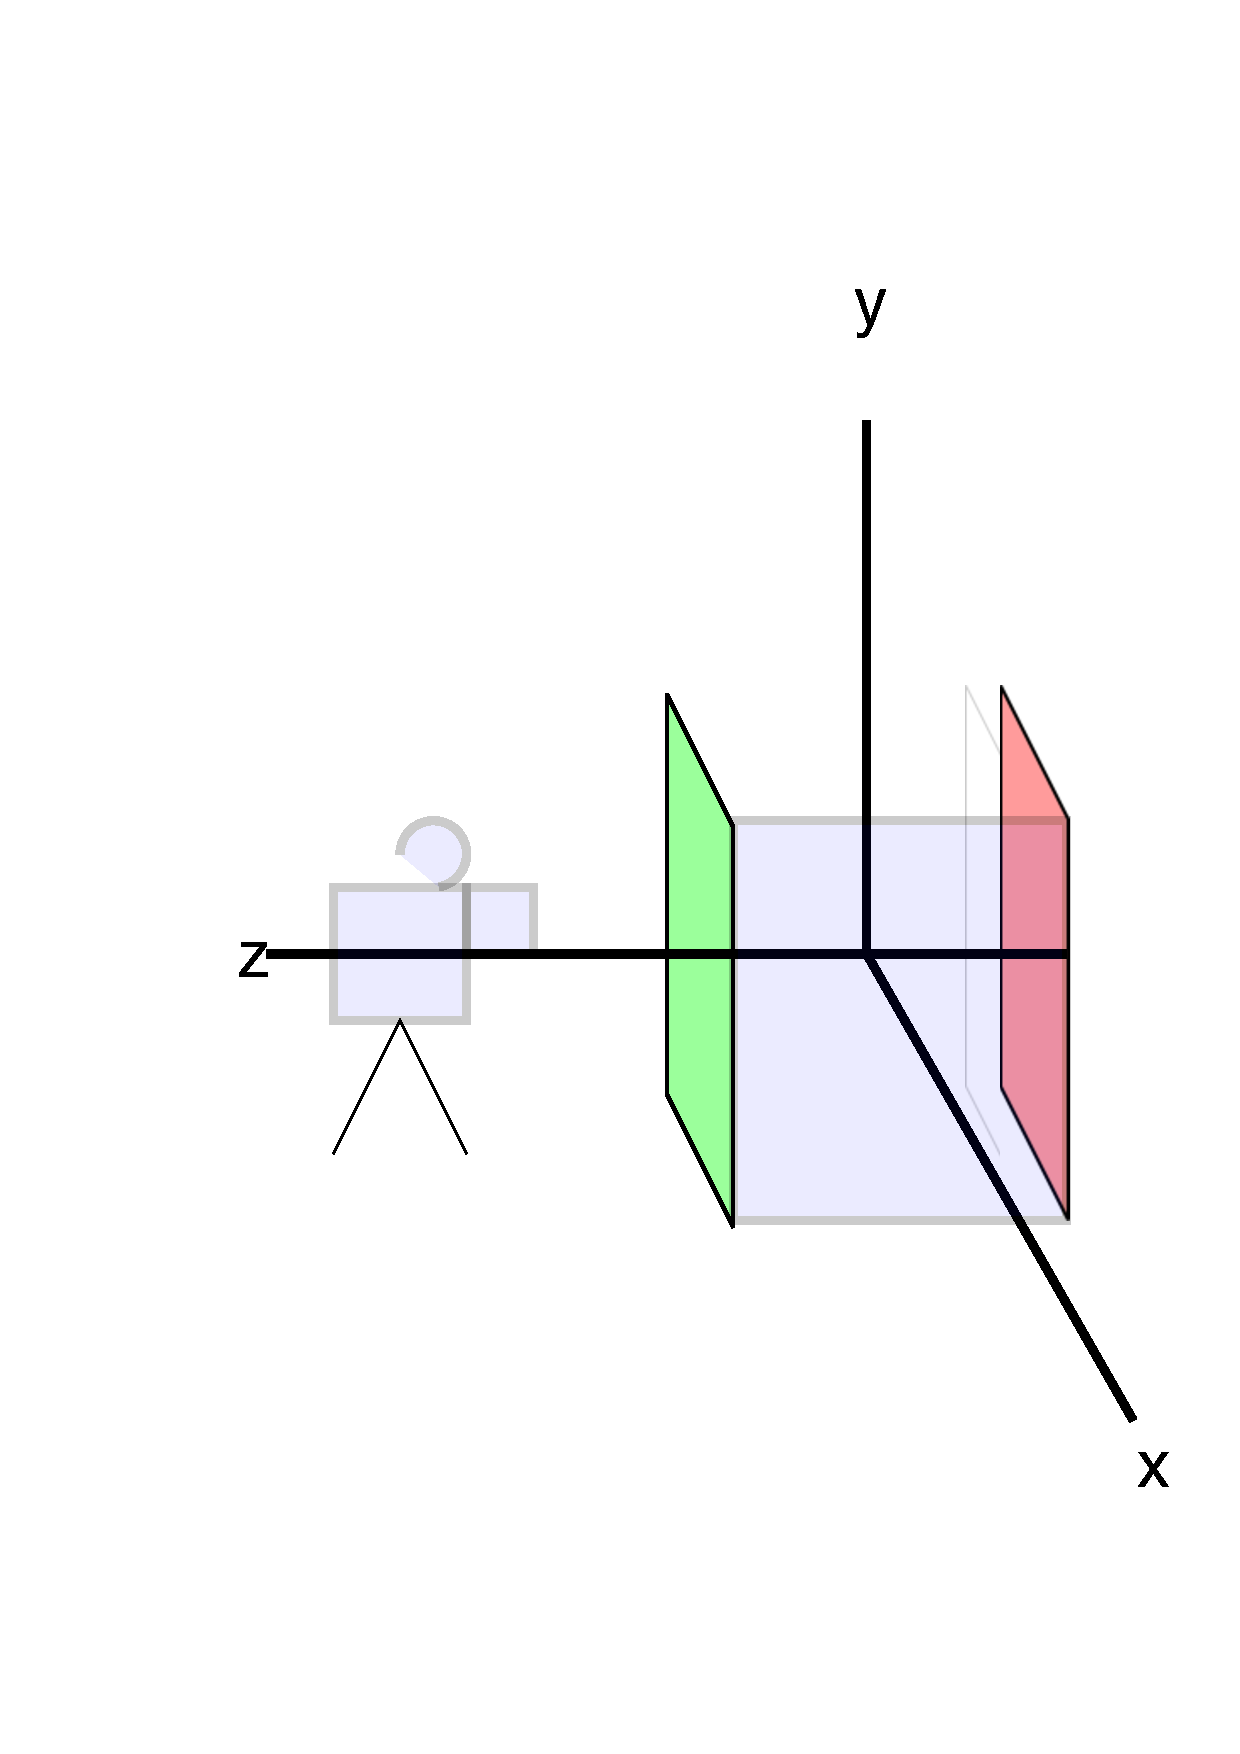
\includegraphics[width=0.4\textwidth]{cube_construct.pdf}
\end{center}
\caption{A partially built cube.}
\label{fig-cube}
\end{figure}





\end{document}
